\documentclass[french]{article}
\usepackage{graphicx}
\usepackage{caption}
\usepackage[T1]{fontenc}
\usepackage[utf8]{inputenc}
\usepackage{lmodern}
\usepackage{geometry}
\geometry{
	a4paper,
	left=25mm,
	right=25mm,
	top=30mm,
	bottom=30mm,
}
\usepackage{babel}
\usepackage{pgfgantt}



\usepackage[unicode=true,pdfusetitle,bookmarks=true,bookmarksnumbered=false,bookmarksopen=false,
breaklinks=false,pdfborder={0 0 0},backref=false,colorlinks=true,urlcolor=blue]{hyperref}

\graphicspath{{images/}}

\author{Andrea Brugnoli \\ 
\hspace{2.8pt} Docteur ISAE-Supaéro 2020\\
Ingénieur ISAE-Supaéro 2017}
\title{Méthodes numériques pour la révolution digitale des jumeaux numériques: de la modélisation multi-physique haute fidélité aux modèles réduits pour l'ingénierie}

\date{}

\begin{document}

\maketitle

\large{Dossier de candidature au prix de la fondation Jean-Jacques et Félicia
	Lopez-Loreta pour l’excellence académique}


\begin{figure}[h]
	\centering
	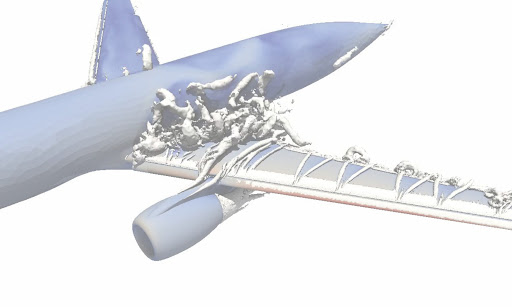
\includegraphics[width=.95\textwidth]{3Dplane.jpg}
	\captionsetup{labelformat=empty}
	\caption{Source: \href{http://www.fenics-hpc.org/}{FEniCS-HPC website}}
\end{figure}





\thispagestyle{empty}

\newpage

\section{Contexte et Objectifs du projet}

\subsection{Le candidat}
La technologie,  les sciences et leur impactes sur l'humain m'ont toujours intéressé. C'est pour cela que j'ai opté pour un baccalauréat littéraire avec option informatique (obtenu en 2011 a Vérone, Italie). Après mon baccalauréat\footnote{En Italie il est possible d'accéder aux universités scientifique après un Bac. L.}, j'ai obtenu une licence en ingénierie mécanique du Politecnico de Milan. Pendant la première année du master en ingénierie Spatiale, j'ai décide de partir \`a l'étranger et j'ai choisi d'effectuer un double diplôme a l'ISAE-SUPAERO. J'ai pu approfondir mes connaissances en automatique grâce \`a un master recherche en collaboration avec Supélec/Université Paris Saclay, ainsi que mes compétences en mathématiques appliquées \`a travers un parcours specilis\'e. Mon intérêt pour les systèmes dynamiques et la simulation m'a amené au centre national d'études spatiales (CNES) pour mon stage de fin études, ou j'ai effectué des simulations intensives sur le supercalculateur. \\

J'ai donc décidé de poursuivre un doctorat de recherche dans l'automatique et les mathématiques appliques (calcul numérique), au sein du projet INFIDHEM (Interconnected Infinite-Dimensional Systems for Heterogeneous Media). Le projet consistait a utiliser un formalisme mathématique capable de traiter d'une manière unifiée les problèmes multi-physique. Mon travail était centre sur la modélisation et discrétisation des structures flexibles minces, très utilisées dans l'aéronautique (cf. Fig \ref{fig:IntRod}). Mes travaux de thèse ont été présentés devant un jury international (Thomas Hélie, directeur de Recherches DR2 au CNRS, Yann Le~Gorrec, Professeur ENSMM et Alessandro Macchelli, professeur associé \`a l'Universit\'e de Bologne) et ont été diffuses \`a travers des conférences internationales et 5 articles de revue rédiges par le candidat \cite{brugnoli2019ammmin,brugnoli2019ammkir,brugnoli2020msd,brugnoli2021ther,brugnoli2021num}. \\

Ma forte curiosit\'e pour les thématiques de ma thèse ne m'a pas abbandon\'e dans la suite. C'est pour cela que j'ai décidé de continuer en Post-Doc \`a l'Universit\'e de Twente, dans un projet qui vise a étendre la compréhension de mécanismes physiques sous-jacents le vol biologique (en particulier les oiseux). Mon rôle consiste \`a mettre en place des algorithmes numérique capables de reproduire fidèlement la structure physique du problème \cite{califano2021}.

\begin{figure}[hbt]
	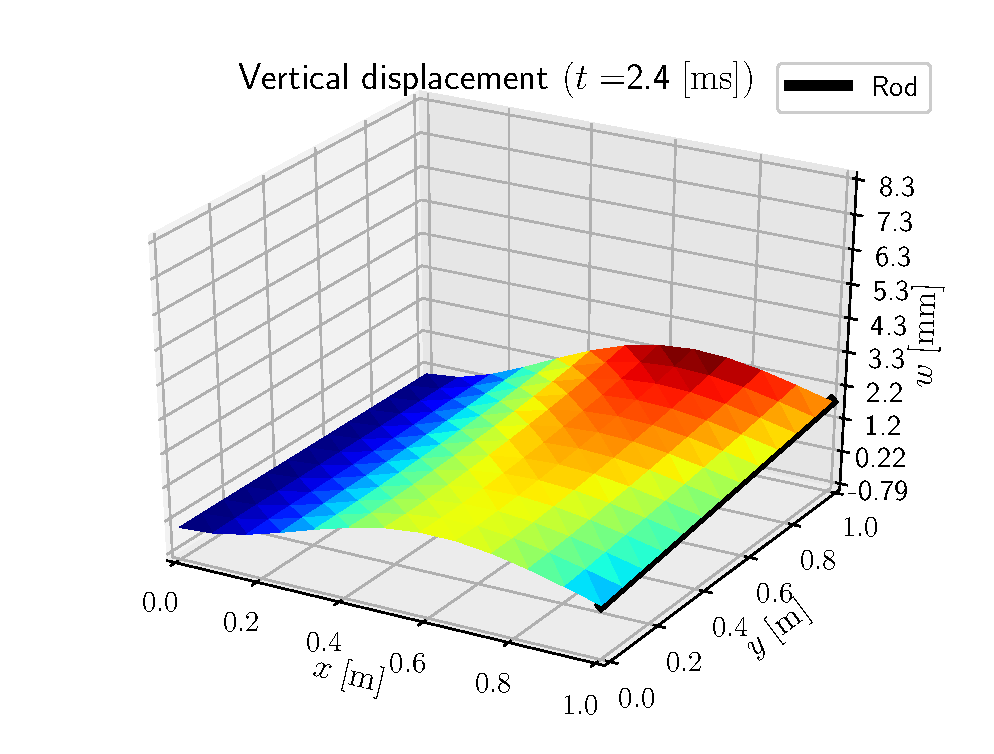
\includegraphics[width=0.5\linewidth]{SnapRod_t25.eps}
	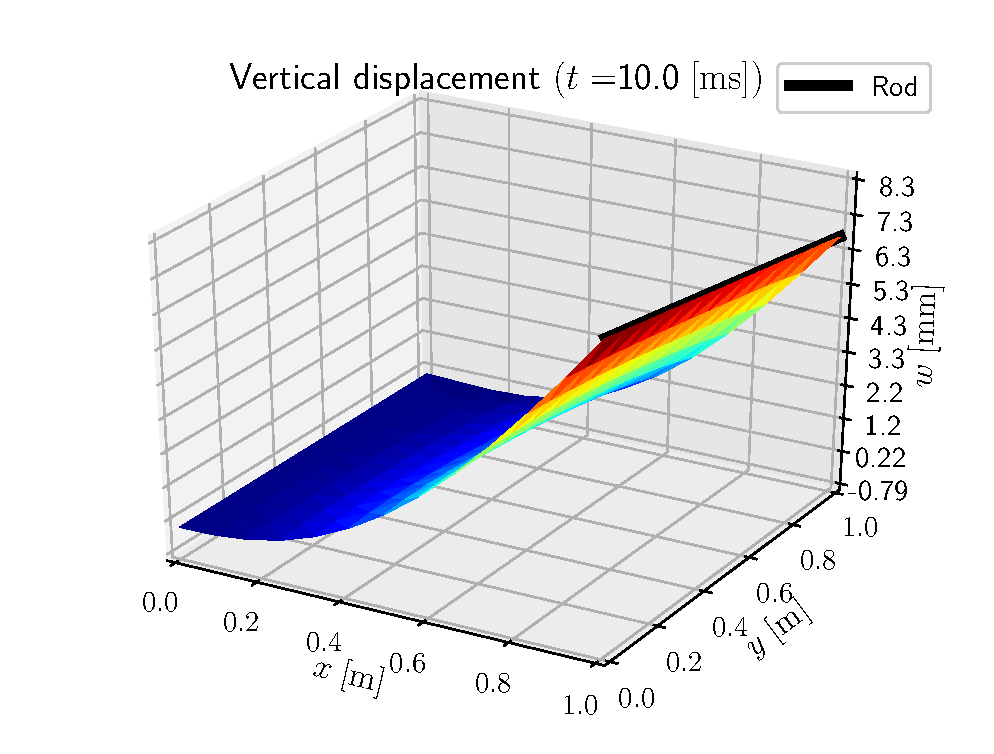
\includegraphics[width=0.5\linewidth]{SnapRod_t100.eps}
	\caption{Simulation d'une plaque mince flexible connectée \`a une poutre rigide.}
	\label{fig:IntRod}
\end{figure}



\subsection{Contexte}

\begin{figure}[tb]
	\centering
	\includegraphics[width = \textwidth]{Bird_Port_Hamiltonian_Subsystems_FULL_ARC.eps}
	\caption{Modèle d'un oiseau robotique bio-inspiré vu comme l'interconnexion de plusieurs systèmes dynamiques. }
	\label{fig:pH_view_bird}
\end{figure}


Ma thèse s'est inscrite dans le cadre d'un projet européen financé par l'agence national de la recherche (ANR) et la Fondation allemande pour la recherche (DFG). L'ambition du projet était de pousser la compréhension d'un formalisme mathématique issu de la physique et de la théorie des systèmes pour le traitement unifié des applications divers (mécanique des solides, des fluides, l'électromagnétisme et la thermodynamique). Il s'agit du formalisme port-Hamiltonien, bas\'e sur la mécanique Hamiltonienne et les graphe de liaisons pour la modélisation des systèmes dynamiques. Il y a 30 ans, le premier article sur cette théorie était publi\`e. Dans le cadre de ma thèse, j'ai pu contribuer \`a étendre ce formalisme envers les applications, en développant des modèles mathématiques et numériques pour la mécanique des solides \cite{brugnoli2019ammmin,brugnoli2019ammkir}, la mécanique multi-corps flexibles~\cite{brugnoli2020msd} et la thermoelasticit\'e~\cite{brugnoli2021ther}. \\

Aujourd'hui ce formalisme a désormais atteint le niveau de maturit\'e pour attaquer les application industriel. Il en est convaincu Volker Mehrmann, vice-président de la société mathématique européenne (EMS), qui a illustré les advantages de ce formalisme dans une \href{https://meetings.siam.org/sess/dsp_programsess.cfm?SESSIONCODE=70329}{conférence plénière} a l'occasion de la SIAM Conference on Computational Science and Engineering. Ce niveau de maturit\'e est aussi témoigné par le fait que le conseil de la recherche européen (ERC) \`a récemment attribu\'e \`a Stefano Stramigioli une subvention de 2.8 millions d'euros pour le projet \href{http://www.portwings.eu/}{Portwings}. Ce projet, dans le quel je suis impliqu\'e pour mon post-doc, cherche \`a améliorer la compréhension du vol battu pour pouvoir perfectionner le design et la construction des robot biomimétiques. L'ambition réside dans le fait d'utiliser la théorie port-Hamiltonien pour expliquer les interactions complexes entre l'aérodynamique et la flexibilit\'e de l'aile (cf. Fig. \ref{fig:pH_view_bird}). \\

De plus en plus, on entend parler des jumeaux numériques (digital twins) comme une ressource fondamental de l'industrie 4.0. Plusieurs acteurs se sont mobilités pour développer leur expertise, comme par exemple Siemens et Dassault. Pour réaliser un développement substantiel dans les domaines d'application les plus critiques pour la société, des investissements considérables seront nécessaires dans les méthodes mathématiques et informatiques qui sous-tendent les jumeaux numériques : en particulier il faudra disposer  des techniques de déploiement robustes, rapides et accessibles \cite{niederer2021}. Étant donné le potentiel du formalisme port-Hamiltonien pour les traitement unifié des problèmes multiphysiques \`a travers différentes échelles et précision, il est possible que son adoption en industrie facilitera cette révolution digitale. 


\subsection{Le projet}
Dans ce projet de recherche, le but consiste \'a mettre en place des méthodes numérique pour accélérer la simulation des problèmes fluide-structure d'un facteur 100, par rapport au temps de calcul demandé par une simulation haute-fidélité.  Une éventuelle réussite permettra donc d'intégrer des modèles physique plus économique, qui pourront remplacer des simulations très couteuse et ainsi faciliter le design et la prise des décisions. L'accélération des codes de calcul pour la simulation numérique est considéré un défis fondamental pour faire avancer le niveau technologique de l'industrie aérospatiale (cf. par exemple  le programme de digitalisation d'AIRBUS \href{https://www.airbus.com/innovation/industry-4-0/digital-design-and-manufacturing-ddms.html}{DDMS}).   \\

Un défis fondamental des modèles réduit est la capacité \`a représenter des physique extrêmement complexes d'une manière précise. 
Dans un premier temps, des simulations haute fidélité seront donc mise en place. Ces modèles numériques devront retenir les propriété physique du problème (conservation d'énergie global, tracement des échanges des énergies entre différents systèmes, conservation d'invariants du problème). Dans un second temps, des technique issus de l'intelligence artificielle seront utilisés pour obtenir des modèles réduit (une technique très prometteuse en ce sens est présentée dans \cite{lee2020}). Dans cette phase, l'impérative reste la fidélité a la physique des modèles ainsi obtenu~\cite{willcox2021}. Le dernière objectif consistera \`a utiliser des modèles réduit pour optimiser le design mécanique des structures et vérifier la validité des modèles réduits.\\

La vision derrière ce projet est que l'utilisation des algorithmes fidèles \`a la structure physique du problème pourra dramatiquement améliorer les techniques normalement utilisées pour la réduction du modèles et l'optimisation. La structure physique du problème est normalement ignorée par les algorithmes de réduction, qui traitent les simulations comme des black-box. Le modèles réduits respectueux de la physique sont extrêmement plus précis des ceux qui ne garantissent pas le respect de la physique sous-jacent \cite{lee2020}. Les modèles ainsi obtenu pourront être utilisés en industrie pour réduire les  co\^{u}ts associés au design, l'optimisation et le monitorage en cours de vie.

\section{Organisation du projet}

\subsection{Structure generale du projet}

Les projet de recherche sera structures en trois macro tâches:
\begin{enumerate}
	\item Développement des algorithmes numériques haute-fidélité pour problèmes d'interaction fluide-structures. Cet algorithme devront respecter les échanges d'énergie entre sous-systèmes et les invariants du problème.
	\item Méthodes de réduction garantissant le respect de la structure physique. Cela concerne les invariants du problèmes ainsi que la séparation entre notions topologique (i.e. topologie du maillage pour chaque domaine physique et  de l'interconnexion) et métrique (i.e. géométrie du maillage).
	\item Design optimal basés sur les méthode haute fidélité et réduits. Cette étape permettra de évaluer l'efficacit\'e de l'approche propos\'e.
\end{enumerate}

Le modèles réduit seront plus rapides mais inévitablement moins précis par rapport aux simulations fines. Achever ces trois macro-tâches permettra de comprendre le compromis entre temps de calcul et précision pour des applications d'intérêt industriel. 

\subsection{Moyens et partenariats}
Pour ce que il concerne la mise en place du projet, des différents partenariat en France et \`a l'international seront mis en place. Pour ce qui concerne les aspect théorique fondamentaux Bernhard Maschke (Universit\'e de Lyon), Arjan van der Schaft (University of Groningen) et Stefano Stramigioli (University of Twente) constitueront les interlocuteurs académiques principaux. \\

Pour ce qu'il concerne la première macro-tâche, il sera possible de reprendre le travail effectuer dans le cadre de ma thèse, qui a donn\'e lieu a un code de calcul pour application multiphysique (le code SCRIMP décrit dans~\cite{brugnoli2021num}). Ce code sera ultérieurement développé pour traiter des problèmes d'interaction fluide-structure. Pour ce qui concerne la préservation de la physique au sein des algorithmes, des collaborations avec Marc Gerritsma (département d'aérodynamique de l'Universit\'e de Delft) seront mises en place. Pour ce qui concerne l'interaction fluido-structure, l'office National d'Études et de Recherches Aérospatiales (ONERA) vante une profonde expertise en ce domaine et représentera l'interlocuteur principal pour les problèmes liés au couplage multiphysique. 
\\


Pour ce qui concerne la deuxième macro-tâche, i.e. la réduction des modèles, il sera possible de mettre en place des collaboration avec Charles Poussot-Vassal (chercheur principal \`a l'ONERA),  Volker Mehrmann (TU Berlin) et Paul Kotyczka (TU Munich). \\
 
Pour la troisième partie, il sera important de dialoguer avec Joseph Morlier (ISAE-Supa\'ero et Institut Clément Ader).
 

\subsection{Le plan et livrables}

Chaque macro-tâche est directement associ\'ee \`a une thèse. Pour cela les recrutement des trois thésards et d'un post doc est prévu, ainsi que la coopération des trois chercheurs. Chacun entre eux sera affect\'ees \`a chaque macro-sujet:
\begin{itemize}
\item développement du code pour calcul scientifique;
\item développement du code pour la partie intelligence artificielle;
\item expertise pour l'optimisation multidisciplinaire.
\end{itemize} 
\begin{figure}[h!]
	\begin{center}
	\begin{ganttchart}[y unit title=0.6cm,
		y unit chart=0.6cm, 
		x unit=0.4cm,
		vgrid,hgrid, 
		title label anchor/.style={below=-1.6ex},
		title left shift=.05,
		title right shift=-.05,
		title height=1,
		progress label text={},
		bar height=0.7,
		group right shift=0,
		group top shift=.6,
		group height=.4]{1}{30}
		%labels
		\gantttitle{Dur\'ee totale}{30} \\
		\gantttitle{$T_0 + 12$}{6} 
		\gantttitle{$T_0 + 24$}{6} 
		\gantttitle{$T_0 + 36$}{6} 
		\gantttitle{$T_0 + 48$}{6} 
		\gantttitle{$T_0 + 60$}{6} \\
		%tasks
		\ganttbar{Partenariats}{1}{2} \\
		\ganttbar{Code SCRIMP}{1}{1} \\
		\ganttbar{1$^\circ$ th\`ese}{4}{21} \\
		\ganttbar{2$^\circ$ th\`ese}{10}{27} \\
		\ganttbar{3$^\circ$ th\`ese}{13}{30} \\
		\ganttbar{Post-Doc}{16}{27} \\
		\ganttbar{Soutenances}{22}{30} \\
		\ganttbar{Dissémination}{28}{30} 
		%relations 
		\ganttlink{elem0}{elem2} 
		\ganttlink{elem1}{elem2} 
		\ganttlink{elem1}{elem3} 
		\ganttlink{elem1}{elem4} 
		\ganttlink{elem1}{elem5}
		\ganttlink{elem2}{elem5}
		\ganttlink{elem3}{elem5}
	\end{ganttchart}
	\end{center}		
\end{figure}

\`A la fin du projet, le livrable consistera en un code capable de modéliser des problèmes multiphysiques et de générer des modèles réduits utilisable \'a la place des modèles haute fidélité.

\subsection{Budjet}
\begin{center}
\begin{tabular}{|c|c|}
	\hline
	D\'epense & Co\^{u}t \\
	\hline
	3 doctorants (temps plein) & $3\times 3\times 40000=360000$  \\
	1 Chercheur ISAE (temps plein) & $5\times 500000=250000$ \\
	1 Post-Doc (temps plein) & $2\times 45000=90000$ \\
	2 Chercheurs ISAE (temps partiel)& $2\times 70000$ \\
	1 Chercheur Onera (temps partiel)& $1\times 70000$ \\
	Matériel  et calcul HPC & $50000$ \\
	Frais annexes (conferences, workshops) & $40000$ \\
	\hline
	\textbf{Total} & 1000000 \\
	\hline
\end{tabular}
\end{center}




\bibliographystyle{unsrt}
\bibliography{biblio_articles}

\end{document}
